\documentclass{beamer}

\mode<presentation>
{
  \usetheme{Hannover}

  \setbeamercovered{transparent}
}


\usepackage[english]{babel}
\usepackage[utf8]{inputenc}
\usepackage{graphicx} 
\usepackage{subcaption}
\usepackage{tikz} 


\title[Pulse Watcher]
{Java Advanced - Short Burst Project}

\subtitle
{Pulse Watcher}

\date{December 1, 2023}

\institute[Universities of Somewhere and Elsewhere]
{
  EHB\\
  Brussels}

\pgfdeclareimage[height=0.5cm]{university-logo}{ehb-logo.jpg}
\logo{\pgfuseimage{university-logo}}

% Delete this, if you do not want the table of contents to pop up at
% the beginning of each subsection:
\AtBeginSubsection[]
{
  \begin{frame}<beamer>{Outline}
    \tableofcontents[currentsection,currentsubsection]
  \end{frame}
}

\begin{document}

\begin{frame}
  \titlepage
\end{frame}


% Structuring a talk is a difficult task and the following structure
% may not be suitable. Here are some rules that apply for this
% solution: 

% - Exactly two or three sections (other than the summary).
% - At *most* three subsections per section.
% - Talk about 30s to 2min per frame. So there should be between about
%   15 and 30 frames, all told.

% - A conference audience is likely to know very little of what you
%   are going to talk about. So *simplify*!
% - In a 20min talk, getting the main ideas across is hard
%   enough. Leave out details, even if it means being less precise than
%   you think necessary.
% - If you omit details that are vital to the proof/implementation,
%   just say so once. Everybody will be happy with that.

\section{Context}

\subsection{Basic Problem}

\begin{frame}{Process monitoring}
  \begin{itemize}
  \item
    Use \texttt{itemize} a lot.
  \item
    Use very short sentences or short phrases.
  \end{itemize}
\end{frame}

\begin{frame}{Features \& Technologies}

  You can create overlays\dots
  \begin{itemize}
  \item using the \texttt{pause} command:
    \begin{itemize}
    \item
      First item.
      \pause
    \item    
      Second item.
    \end{itemize}
  \item
    using overlay specifications:
    \begin{itemize}
    \item<3->
      First item.
    \item<4->
      Second item.
    \end{itemize}
  \item
    using the general \texttt{uncover} command:
    \begin{itemize}
      \uncover<5->{\item
        First item.}
      \uncover<6->{\item
        Second item.}
    \end{itemize}
  \end{itemize}
\end{frame}


\subsection{Examples}

\begin{frame}{Grafana}

\begin{figure}
\begin{subfigure}[h]{0.65\linewidth}
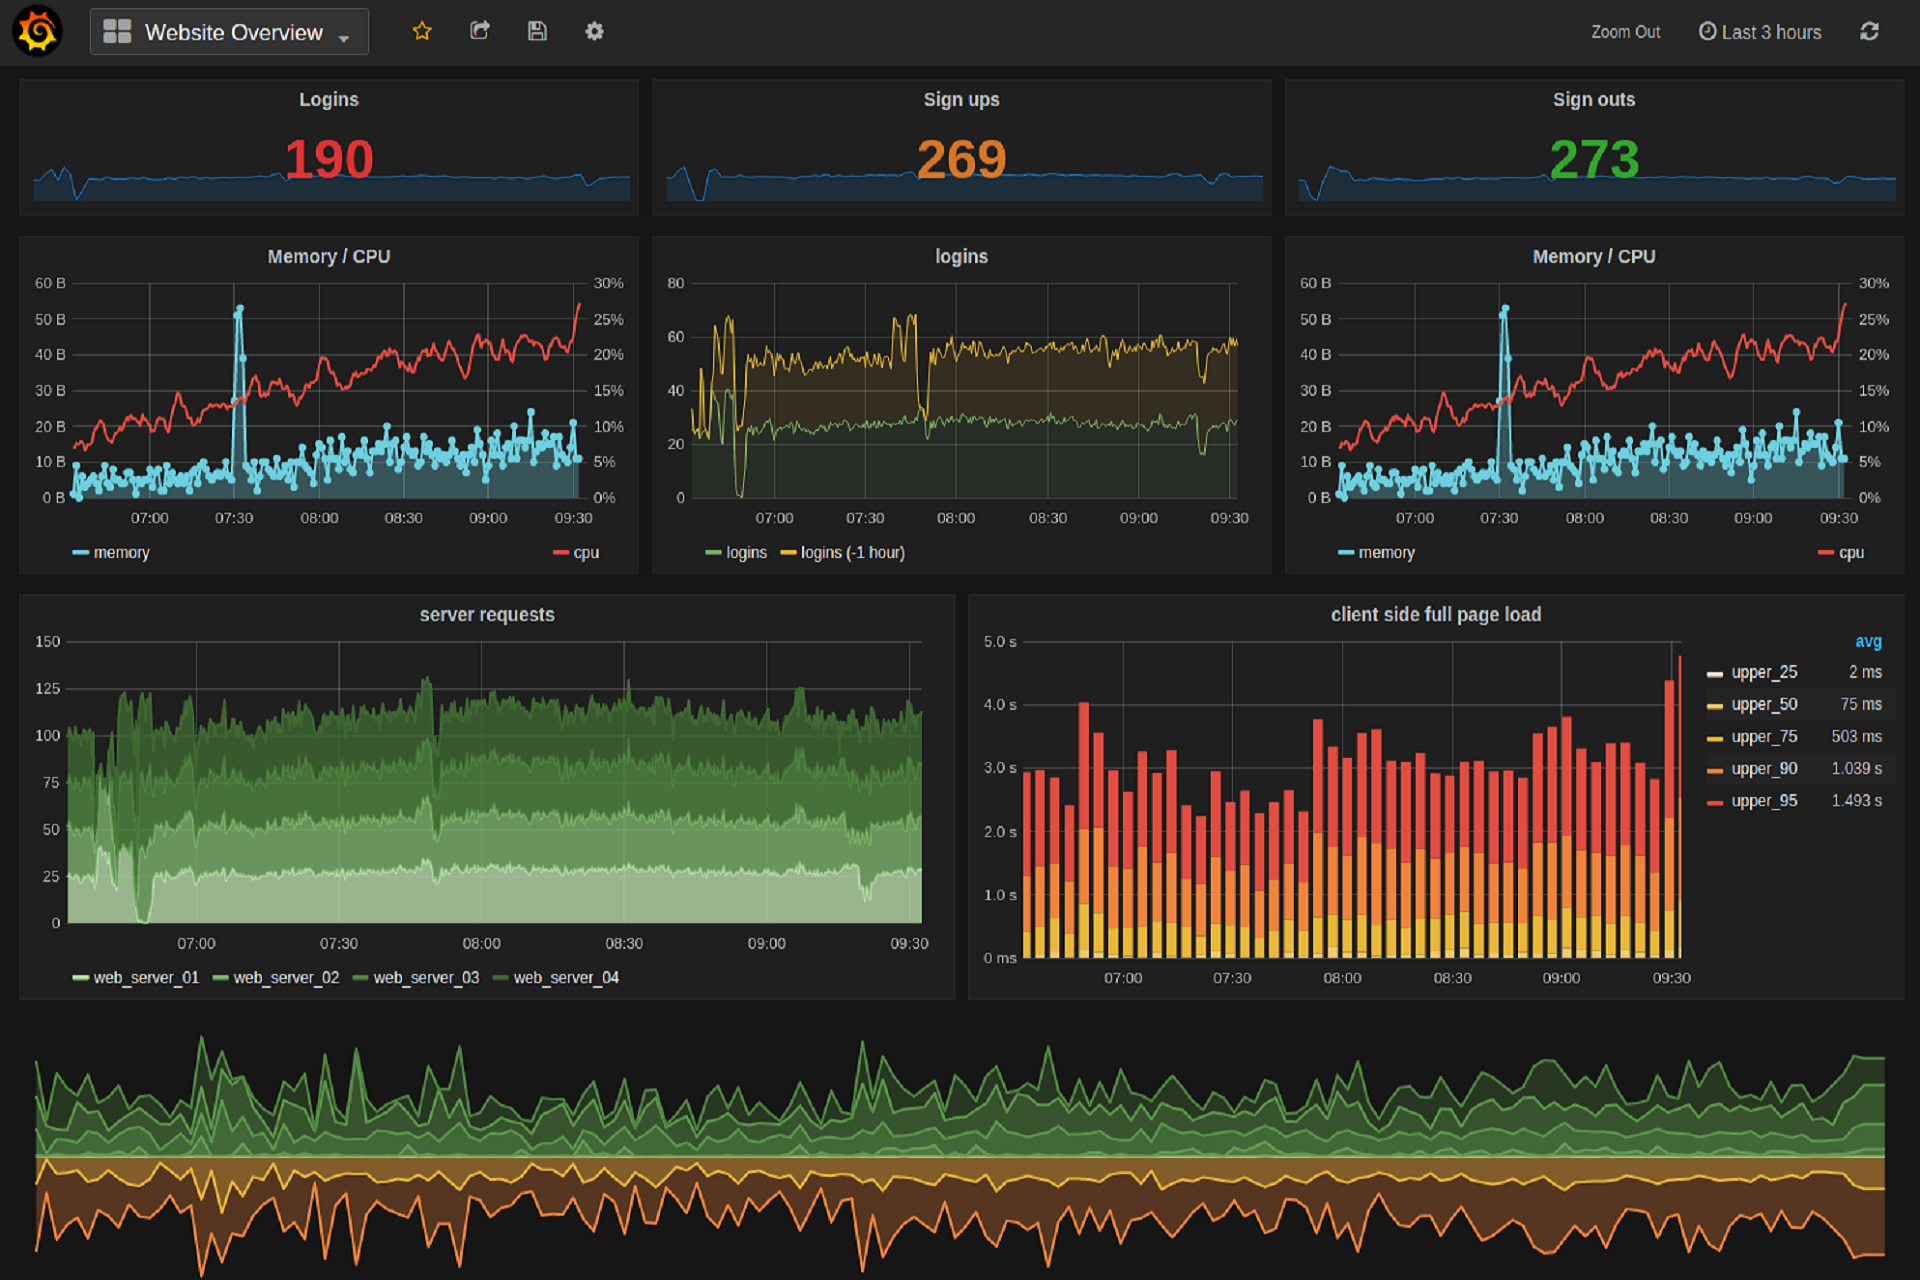
\includegraphics[width=\linewidth]{grafana.png}
\caption{Grafana Dashboard}
\end{subfigure}
\begin{subfigure}[h]{0.3\linewidth}

\includegraphics[width=\linewidth]{prometheus.png}
\caption{Prometheus logo}
\end{subfigure}
\end{figure}

\end{frame}

\section{Pulse Watcher}

\subsection{Demo}

\begin{frame}{Web UI}{Vue.js}
\end{frame}

\begin{frame}{Web UI}{Vue.js}
\end{frame}

\subsection{Implementation}

\begin{frame}{Backend}{Springboot}
% meme - starter pack
% Annotations
% Hide all implementation
\end{frame}

\begin{frame}{Backend}{Server $<$-$>$ Client Web Socket}
% Show Java code
\end{frame}

\begin{frame}{Backend}{Life cycle}

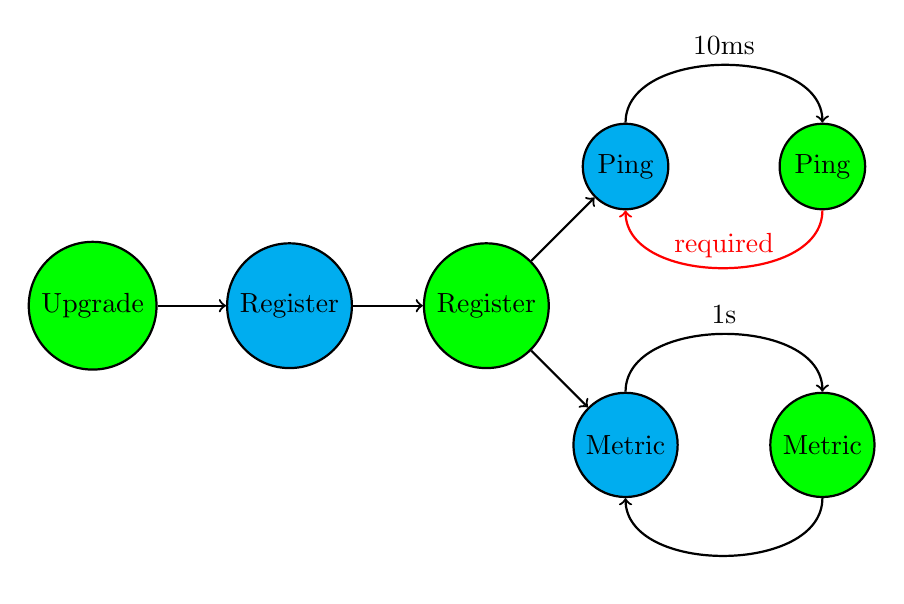
\begin{tikzpicture}[
node distance={25mm},
thick,
client/.style = {draw, circle, fill=green},
server/.style ={draw, circle, fill=cyan} ] 
\node[client] (1) {Upgrade};
\node[server] (2) [right of=1] {Register};
\node[client] (3) [right of=2] {Register};

\node[server] (4) [above right of=3] {Ping};
\node[client] (5) [right of=4] {Ping};

\node[server] (6) [below right of=3] {Metric};
\node[client] (7) [right of=6] {Metric};

\draw[->] (1) -- (2);
\draw[->] (2) -- (3);
\draw[->] (3) -- (4);
\draw[->] (3) -- (6);
\draw[->] (4) to [out=90, in=90] node[midway, above] {10ms} (5);
\draw[->,color=red] (5) to [out=270, in=270] node[midway,above] {required} (4);
\draw[->] (6) to [out=90, in=90] node[midway, above] {1s} (7);
\draw[->] (7) to [out=270, in=270] (6);

\end{tikzpicture}

\end{frame}

\begin{frame}{API}{Protobuffers}
% Show change config packet
% Show short protofbuf def and list advantages
\end{frame}



\section*{Summary}

\begin{frame}{Summary}

  % Keep the summary *very short*.
  \begin{itemize}
  \item
    The \alert{first main message} of your talk in one or two lines.
  \item
    The \alert{second main message} of your talk in one or two lines.
  \item
    Perhaps a \alert{third message}, but not more than that.
  \end{itemize}
  
  % The following outlook is optional.
  \vskip0pt plus.5fill
  \begin{itemize}
  \item
    Outlook
    \begin{itemize}
    \item
      Something you haven't solved.
    \item
      Something else you haven't solved.
    \end{itemize}
  \end{itemize}
\end{frame}



% All of the following is optional and typically not needed. 
\appendix
\section<presentation>*{\appendixname}
\subsection<presentation>*{References \& Documentation}

\begin{frame}[allowframebreaks]
  \frametitle<presentation>{Bibliography}
    
  \begin{thebibliography}{10}
  
  \setbeamertemplate{bibliography item}[online]	

  \bibitem{protobuf-docs}
    Google LLC
    \newblock {\em Protocol Buffers - \url{https://protobuf.dev/}}.
    \newblock \textcopyright 2023
 
  
  \bibitem{vue-docs}
    Evan You
    \newblock {\em Vue.js - \url{https://vuejs.org/}}
    \newblock \textcopyright 2023
  \end{thebibliography}
\end{frame}

\end{document}


